\documentclass[11pt,a4paper]{article}

% 中文宏包
\usepackage{CJK,indentfirst} % 中文设置宏包indenfirst宏包允许设置首行缩进

%伪代码包
\usepackage{algorithm}
\usepackage{algorithmic}

%插入图片
\usepackage{graphicx}

% 数学宏包
\usepackage{latexsym}
\usepackage{bm}
\usepackage{amsmath}
\usepackage{amssymb}

% 插入程序源代码宏包
\usepackage{listings} % 程序代码宏包
\usepackage{xcolor} % 程序代码颜色宏包

%\begin{CJK*}{UTF8}{gbsn}%用宋体
%\end{CJK*}

\begin{titlepage}
\begin{CJK*}{UTF8}{gbsn}%用宋体
	\title{$R^{n}$\footnote{$0.0<R<99.999,\qquad0<n<25$} 高精度计算的简单实现\footnote{此题同北京大学ACM题库1001题}\footnote{本文档的tex文件可在本人的github上找到https://github.com/zhuxu/tex\_file}}
\author{\\ \\ \\ \\ 朱旭\\ \\12720629\\ \\计算机应用技术\\ \\组合数学论文}
\date{2013年12月22日}
\end{CJK*}
\end{titlepage}

\begin{document}
\begin{CJK*}{UTF8}{gbsn}%用宋体

\lstset{numbers=left,
	numberstyle=\tiny,
	keywordstyle=\color{blue}, % 设置关键字颜色
	commentstyle=\color[cmyk]{1,0,1,0}, % 设置评论风格
	frame=single, 
	escapeinside=``, % 设置逃逸字符
	breaklines, %自动折行
	extendedchars=false,
	xleftmargin=2em,xrightmargin=2em, aboveskip=1em, %设置边距
	tabsize=4,
	showspaces=false % 不显示空格
}

\maketitle
\newpage %开始新的一页

\renewcommand{\abstractname}{摘\qquad 要} % 将abstract重命名为 摘要
\begin{abstract}
这里主要介绍了,在计算机上实现高精度计算。我们知道由于计算机语言类型的限制,以C语言为例,每种类型都有一个上限值,所以要进行高精度计算的话极有可能会发生溢出,导致计算失败。这里利用最基本进位方法,同时辅助存储小数点的位置实现可靠的高精度计算。
\end{abstract}

\section{设计分析}
首先设置num\_buffer数组用于存储原始数据,设置num\_input数组用于计算中间值,设置num\_ans用于存储计算结果,设置count变量存储需要计算的次数。num\_buffer,num\_input,num\_ans数组存储数据时,数据的每位数均以字符形式存储。
\newline\indent计算方法:以基本的进位思想,首先从最低位开始,这里以乘法为例,首先将num\_buffer,num\_input两个数组的最低位由字符类型char转换成整数类型int,将这两个数值相乘
得出进位和保留位,将进位转换成char类型存储到num\_input次最低位中,将保留位存储到num\_input中原先用于计算的那个最低位中。以此循环计算,只要有进位就向高位进位即可。
\section{算法描述}
\begin{algorithm}
\caption{Calculate\qquad$y=R^n$}
\begin{algorithmic}
\REQUIRE $0.0<R<99.999\qquad0<n<25$
\ENSURE $y = R^n$
\STATE $len\_buffer \leftarrow strlen(num\_buffer)$
\STATE $len\_input \leftarrow strlen(num\_input)$
\STATE $len\_ans \leftarrow len\_buffer + len\_input$
\FOR{$i \leftarrow len\_buffer\qquad to\qquad0$}
\FOR{$j \leftarrow len\_input\qquad to\qquad0$}
\STATE $num\_ans[i+j+1] += (num\_buffer[i]*num\_input[j])\%10$
\STATE $num\_ans[i+j] += (num\_buffer[i]*num\_input[j])/10$
\ENDFOR
\FOR{$k \leftarrow len\_ans-1\qquad to\qquad 1$}
\IF{$num\_ans[k]  >= 10$}
\STATE $num\_ans[k-1]  += num\_ans[k]/10$
\STATE $num\_ans[k]  \%=10$
\ENDIF
\ENDFOR
\ENDFOR
\end{algorithmic}
\end{algorithm}
时间复杂度为O(len\_buffer*len\_input),由于len\_input数组由进位产生的故最大为len\_buffer*n,由于这只是计算一次的代价,总的代价需要计算m次,所以总的时间复杂度位O(len\_buffer*m*n),由于将一个双精度数字变为字符形式存储所需要的字符数组的最大长度是个常数,故最终的时间复杂度为$O(n*m)$
\section{运行结果示例}
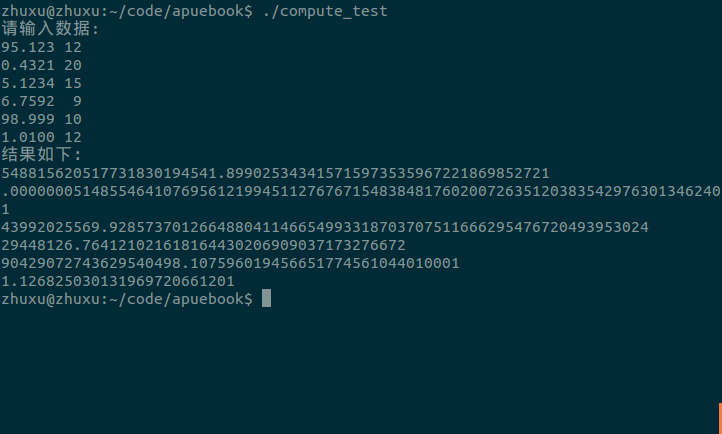
\includegraphics[width=5in]{ans.png}
\section{优化及改进}
在本示例中,并没有考虑到n为偶数或奇数的情况,这里我们考虑n为偶数的情况(奇数情况相同),如果n为偶数,则在计算时我们可以使用一些加速计算的方法。
\newline\indent在num\_buffer计算过第一次之后,可以将num\_input中保存的结果作为第二次计算的初始值,这样我们只需要$lg(n)$次计算便能计算出相应的结果,
奇数情况则需要多计算一次即可,故改进后的总的时间复杂度位$O(mlgn)$

\section{附录}
程序代码如下
\begin{lstlisting}{language=C}
#include <stdio.h>
#include <stdlib.h>
#include <string.h>
#include <ctype.h>

struct node{
	char num_str[126];
	int num;
	struct node *next;
};

int str_mul (char num_buffer[], char num_input[], char num_ans[]);
int str_to_num (char buffer[]);
struct node *sll_reverse (struct node *head);

int main (void)
{
	char buffer[7] = { 0 };
	int count;
	int point_num = 0;
	char num_ans[126];

	struct node *phead = NULL;

	while (scanf ("%s %d", buffer, &count) == 2) {
		buffer[6] = '\0';
		point_num = str_to_num (buffer);
		struct node *ptemp = (struct node *) malloc (sizeof (struct node));
		strncpy (ptemp->num_str, buffer, strlen (buffer) + 1);
		ptemp->num = point_num * count;
		while (count > 1) {
			str_mul (buffer, ptemp->num_str, num_ans);
			count--;
		}
		ptemp->next = phead;
		phead = ptemp;
	}

	if (phead->next != NULL)
		phead = sll_reverse (phead);

	struct node *p_index = phead;
	int flag;
	int sum_bit = 0;
	while (phead != NULL) {
		sum_bit = strlen (phead->num_str);
		flag = 0;
		for (count = 125; count > 0; count--) {
			if ((phead->num_str[count] - 48) > 0) {
				if (count < sum_bit - phead->num) {
					phead->num_str[sum_bit - phead->num] = '\0';
					break;
				}
				phead->num_str[count + 1] = '\0';
				break;
			}
		}
		for (count = 0; phead->num_str[count] != '\0'; count++) {
			if ((phead->num_str[count] > 48)
				|| (count == (sum_bit - phead->num))) {
				flag = 1;
			}
			if (count == sum_bit - phead->num)
				putchar ('.');
			if (flag == 1)
				putchar (phead->num_str[count]);
		}
		putchar ('\n');

		phead = phead->next;
	}

	phead = p_index;
	while (phead != NULL) {
		p_index = phead;
		phead = phead->next;
		p_index->next = NULL;
		free (p_index);
	}

	return 0;
}

struct node *sll_reverse (struct node *head)
{	/* `原地逆转单链表` */
	if (head == NULL)
		return head;
	struct node *upper;
	struct node *later;
	upper = head;
	later = head->next;
	upper->next = NULL;
	head = later;
	while (head->next != NULL) {
		head = head->next;
		later->next = upper;
		upper = later;
		later = head;
	}
	later->next = upper;

	return head;
}

/*`计算乘法`*/
int str_mul (char num_buffer[], char num_input[], char num_ans[])
{
	int i, j = 0;
	int j_temp = 0;
	int k = strlen (num_buffer) + strlen (num_input);
	int k_temp = k - 1;

	num_ans[k] = '\0';
	while (--k >= 0) {
		num_ans[k] = '0';
	}
	j = strlen (num_input);
	j_temp = j - 1;
	for (i = 4; i >= 0; i--) {
		for (j = j_temp; j >= 0; j--) {
			num_ans[i + j + 1] +=
				((num_input[j] - 48) * (num_buffer[i] - 48)) % 10;
			num_ans[i + j] += ((num_input[j] - 48) * (num_buffer[i] - 48)) / 10;
		}
		/*`处理进位` */
		for (k = k_temp; k > 0; k--) {
			if ((num_ans[k] - 48) >= 10) {
				num_ans[k - 1] += (num_ans[k] - 48) / 10;
				num_ans[k] = (num_ans[k] - 48) % 10 + 48;
			}
		}
	}
	strncpy (num_input, num_ans, strlen (num_ans) + 1);

	return 0;
}

/*`返回值为小数点后面的位数`*/
int str_to_num (char buffer[])
{
	int bit_num = 0;

	while (*buffer++ != '.') ;
	while (*buffer != '\0') {
		*(buffer - 1) = *buffer;
		buffer++;
		bit_num++;
	}
	*(buffer - 1) = '\0';

	return bit_num;
}

\end{lstlisting}

\end{CJK*}
\end{document}
